\begin{pastexam}[label={px:ntu-108-ee-dsb-09}]{臺大電機所 108 學年度（B）第 9 題}
（是非；答對 4 分，答錯倒扣 4 分）

If $T$ is a BST and both the left and right subtrees of $T$ are AVL trees, then $T$ must be an
AVL tree.
\end{pastexam}

\begin{pastsoln}
答案是 (B)，錯。

AVL 樹要求\textbf{每一個}節點的左右子樹高度差不超過 $1$（資結書第~10.2~節）。 左右子樹各自是
AVL 樹，只保證子樹裡面的節點平衡，根本身的兩邊高度可能差很多。

反例：依序插入 $3, 2, 1$ 的 BST。
\begin{center}
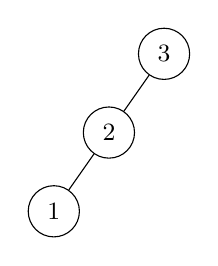
\begin{tikzpicture}[
    every node/.style={circle, draw, minimum size=6.5mm, inner sep=0pt, font=\small},
    level distance=10mm, sibling distance=14mm]
\node {3}
    child {node {2} child {node {1}} child[missing]}
    child[missing];
\end{tikzpicture}
\end{center}
左子樹是以 $2$ 為根、左邊接 $1$ 的樹：節點 $2$ 的左子樹高度 $0$、右子樹是空的（高度 $-1$），
差 $1$；節點 $1$ 是葉子。 所以左子樹是 AVL 樹。 右子樹是空樹，也是 AVL 樹。 但根 $3$ 的左子樹
高度 $1$、右子樹高度 $-1$，差 $2$，所以 $T$ 不是 AVL 樹。 這正是 AVL 插入時要旋轉的 LL 情況。
\end{pastsoln}
